\chapter{DNA sequence classification} \label{sec:dna_sequences}

\section{DNA sequences} \label{subsec:what_are_dna_sequences}

\gls{DNA} is composed of a linear string of nucleotides, or bases, which are referred to by their chemical names' first letters: \gls{A}, \gls{T}, \gls{C}, and \gls{G}. 

\gls{DNA} sequencing is the technique of finding the order of the four bases. Scientists can determine the type of genetic information carried in a \gls{DNA} segment by examining the sequence. Furthermore, and more significantly, sequencing data can reveal mutations in a gene that could lead to illness, by comparing a healthy and a mutated sequence~\cite{2020DNASheet}.

The four chemical bases of the \gls{DNA} double helix always connect with the same partner to produce "base pairs". \gls{A} is always paired with \gls{T}, while \gls{C} is always paired with \gls{G} (Figure~\ref{fig:dna}). This pairing explains the technique by which \gls{DNA} molecules are copied when cells divide, as well as the methods used in most \gls{DNA} sequencing research. The human \gls{genome} is made up of around 3 billion base pairs, which carry the instructions for creating and maintaining a human person~\cite{2020DNASheet}.

\begin{figure}[htbp]
    \centering
    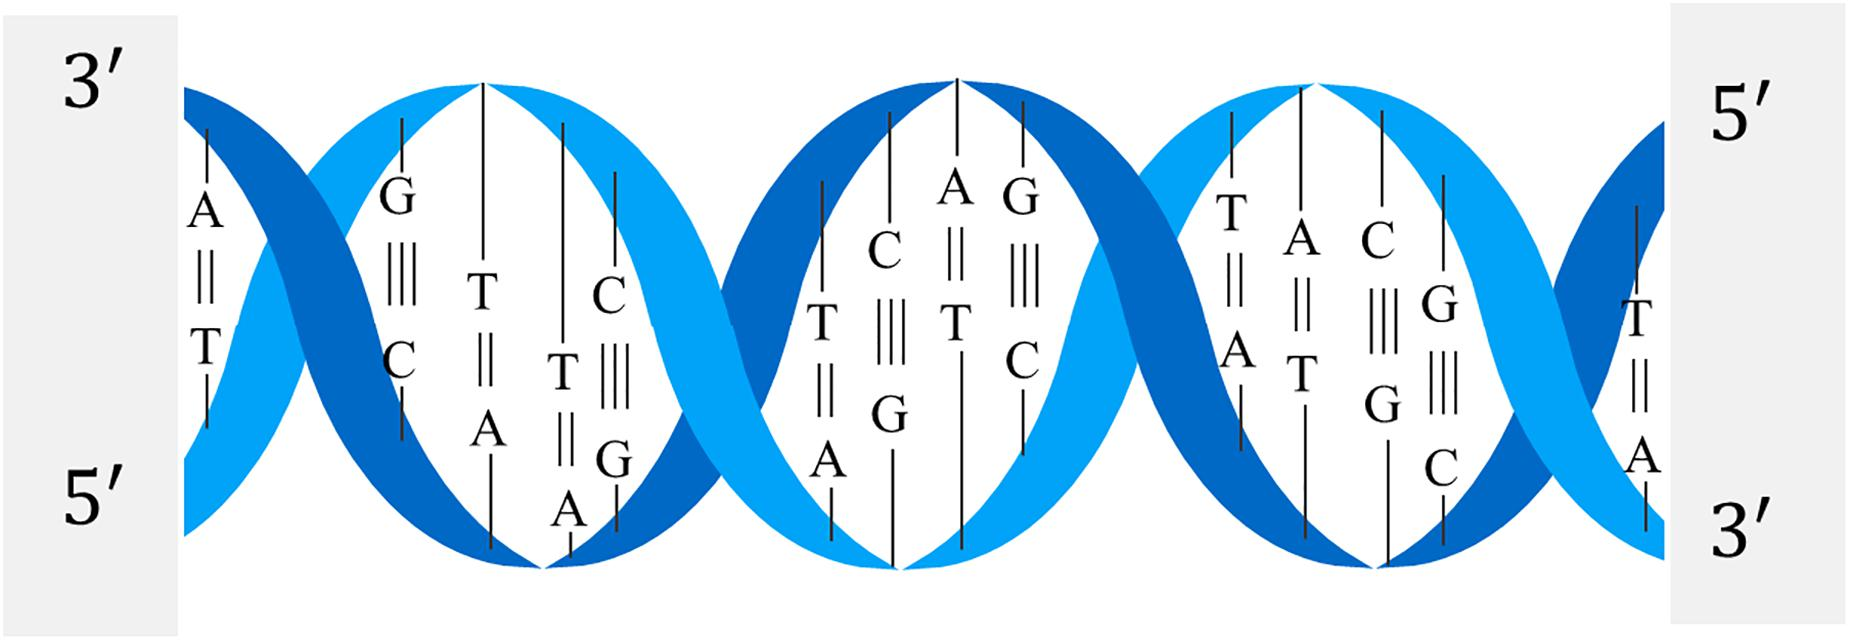
\includegraphics[width=0.5\linewidth]{Chapters/Figures/dna.jpg}
    \caption{Double helix of DNA~\cite{Yang2020ReviewDNA}}
    \label{fig:dna}
\end{figure}

Since the Human Genome Project's completition~\cite{TheProject}, technological advancements and automation have made it possible for individual genes to be sequenced on a regular basis, by reducing the amount of time it takes to perform the sequencing and also reducing its cost. Some labs can sequence over 100,000 billion bases per year, and a few thousand dollars is enough to sequence an entire \gls{genome}~\cite{2020DNASheet}. 

\section{DNA sequence classification - Traditional ML}

The fast development of sequencing technology in the post-genomic era has rapidly increased the amount of biological sequence data. However, structural and functional data from wet-lab investigations are still limited due to the time and cost of the research. Many effective and computationally affordable approaches for analyzing sequence data have recently been presented. Because the majority of sequence analysis tasks are expressed as binary or multiclass classification tasks, \gls{ML} techniques have been playing an important role in these types of  challenges~\cite{Liu2019BioSeq-Analysis:Approaches}.

In \gls{ML}, the goal of classification is to use the training set to create a classification model that can predict the category of unknown incoming samples. \gls{DNA} sequence classification is the process of predicting the kind of \gls{DNA} sequence based on structural or functional similarities, then predicting the sequence function and relationships with other sequences, and finally assisting in the identification of genes in \gls{DNA} molecules~\cite{Yang2020ReviewDNA}.

However, for a \gls{ML} model to be able to predict, it first needs input features, and that is the main problem with sequences. The most difficult component is the feature selection because the sequences only consist of a set of four letters, meaning they lack explicit features. Converting sequences into an effective numerical representation that reflects the underlying relationship with the feature to be predicted can have a big impact on the model's performance~\cite{Chen2020ILearn:Data}.

It is standard practice to encode molecular information as numerical features in order to apply various \gls{ML} algorithms to molecular data. Molecular descriptors are one of the most powerful tools for describing the biological, physical, and chemical features of molecules, and they have been utilized in a variety of research to better understand molecular interactions. These descriptors capture and amplify different features of molecular topology in order to better understand how molecular structure influences molecular properties~\cite{Dong2018PyBioMed:Interactions}. However, it is worth emphasizing that these descriptors need to be manually created, meaning the feature selection is a handcrafted process. Some examples of \gls{DNA} sequence descriptors are the nucleic acid composition, structure composition and sequence length~\cite{Liu2019BioSeq-Analysis:Approaches,Chen2020ILearn:Data,Bonidia2021MathFeature:Descriptors}.

Tools such as \textit{BioSeq-Analysis}~\cite{Liu2019BioSeq-Analysis:Approaches} and \textit{iLearn}~\cite{Chen2020ILearn:Data} are platforms capable of calculating descriptors for not only \gls{DNA} but also \gls{RNA} and protein sequences. In addition, these packages also perform \gls{ML} functions on the calculated features. \textit{BioSeq-Analysis} focuses on automatically completing feature extraction, predictor construction, and performance evaluation. \textit{iLearn} has functions for feature extraction, clustering, feature selection, dimensionality reduction, and ensemble learning, making it a more comprehensive package.

Another important stage in sequence analysis is the creation of predictors. Many \gls{ML} methods have been employed to predict structural and functional characteristics and to help in the annotation of genomic data. \gls{SVM}, \gls{RF}, \gls{ANN}, \gls{KNN}, and \gls{LgR} are some examples of these methods~\cite{Chen2020ILearn:Data}.


%Descriptors 
%Algorithms  

\section{DNA sequence classification - DL}

A common difficulty in data mining is classifying biological sequences as a specific data type. This is a tough challenge, due to the non-numerical properties of biological sequence elements, the sequence interaction between sequence elements, and the variable sequence length~\cite{Yang2020ReviewDNA}. \gls{ML} methods for supervised classification tasks are, without a doubt, heavily reliant on the feature selection stage, and it is required to detect and quantify relevant aspects of the objects to classify in order to develop a suitable representation. \gls{DL} models have recently been shown to be capable of automatically extracting meaningful features from input patterns~\cite{LoBosco2017DeepClassification}. This is possible due to feature learning techniques that \gls{DL} methods possess. These techniques allow the automatic identification of the representations required for feature detection from raw data, meaning that the human feature engineering is removed, and the machine will learn the features instead. As a result, \gls{DL} models only need the sequence itself as input, unlike \gls{ML} models that require the previously calculated features. However, first it is required to transform the string sequence into a numerical value in order to create an input matrix for the model~\cite{Yang2020ReviewDNA}. Sequential encoding, one-hot encoding, and k-mer encoding are three popular methods for sequence encoding~\cite{Choong2017EvaluationMethod} and Table~\ref{tab:encoding_methods} summarizes the differences between them. The encoding technique is also significant for classification accuracy.

\begin{table}[ht]
	\caption{DNA sequence encoding methods~\cite{Yang2020ReviewDNA}}
	\label{tab:encoding_methods}
\centering
\begin{tabular}{lp{8cm}}
	\toprule
	\textbf{Encoding Method} & \textbf{Features} \\
	\midrule
	
	Sequential encoding & Each base is encoded as a number. For example, change [A,T,G,C] to [0.25,0.5,0.75,1.0], and any other character to 0.\\\midrule
	
    One-hot encoding & Each base is encoded as a vector. [A,T,G,C] will become [0,0,0,1],[0,0,1,0],[0,1,0,0],[1,0,0,0]. These vectors can be combined into a 2-dimensional array.\\\midrule
    
    K-mer encoding & Decomposes a sequence into k-length overlapping segments. "ATGCATCGA" becomes "ATGCAT", "TGCATG", "GCATGC", "CATGCA"  when \textit{k}=6 is used. The segments must then be converted to numerical values.\\
    
	\bottomrule
\end{tabular}
\end{table}

In the case of the k-mer encoding method, the encoded sequence is not yet ready to be fed into the model, as the result of the encoding method is not a numerical value. The \gls{DL} model still needs this produced k-mer sentence to be transformed into a dense feature vector matrix and this can be achieved by using a word embedding layer. Word embedding is a technique for assigning each word in a sequence a continuous vector representation, and words with similar meanings are near in distance in the vector space generated.~\citeauthor{Gunasekaran2021AnalysisModels}~\cite{Gunasekaran2021AnalysisModels} used the k-mer encoding to generate segments of \gls{DNA} sequences and then applied the word embedding layer to their model to transform the sentence into a dense feature vector matrix. It is also possible to apply an embedding layer to other encoding methods. Although there is no semantic similarity to uncover, this concept has also been applied at character-level, representing a first step toward completely automated feature learning. For example,~\citeauthor{LoBosco2017DeepClassification}~\cite{LoBosco2017DeepClassification} used \gls{CNN} and \gls{RNN} for the purpose of \gls{DNA} sequence classification. For both models, their first layer was an embedding layer, which accepted as input 16-dimensional one-hot encoding of sequence characters and produced a 10 dimensional continuous vector. The embedding representation may be achieved using a single feed-forward layer using random weights in order to learn embedding for all of the terms in the training dataset.

In Section~\ref{sec:previous_work}, relevant previous work on DNA classification will be provided, and it is possible to conclude that \gls{CNN} and \gls{RNN} are the most commonly used \gls{DL} models.

% (over strings?)
% common architectures